\documentclass[utf8x,14pt, coursreport]{G7-32}
% masterthes -- диссертация магистра
% diploma -- дипломная работа инженера
% bachelor -- квалификационная работа бакалавра
% coursreport -- курсовая работа
% projreport -- курсовой проект по дисциплине
% appreport -- отчет о прикладных научных исследованиях
% scireport -- отчет о научно-исследовательской работе
% report -- отчёт (по практике)
\usepackage[utf8]{inputenc}
\usepackage[english,russian]{babel}
\usepackage{epstopdf}
%\usepackage{bookmark}
\usepackage{titletoc}

\usepackage{verbatim}
\usepackage{fancyvrb}
\usepackage{listings}
\usepackage{listingsutf8}

\lstloadlanguages{C, [ANSI]C++}

\usepackage[colorlinks=true, citecolor=blue, bookmarksopen=true]{hyperref}

% additional packages
%\usepackage{subcaption}
\usepackage{float}
%\usepackage{rotating}
%\usepackage{multirow}
%\usepackage{mdwlist}
\usepackage{textcase}
\usepackage{array}
\usepackage{graphicx}

\usepackage{color}

\definecolor{greencomments}{rgb}{0, 0.3, 0}
\definecolor{redstrings}{rgb}{0.8, 0.0, 0}
\definecolor{orangekeys}{rgb}{0.0, 0.2, 0.8}

% Определим свой цветовой стиль для листинга программ
\lstdefinestyle{cstyle}{
	commentstyle=\color{greencomments},
	stringstyle=\color{redstrings},
	basicstyle=\footnotesize,
	keywordstyle=\color{orangekeys},
	extendedchars=true,
	breaklines=true,
	captionpos=b,
	keepspaces=true,
	numbers=left,
	numbersep=5pt,
	showspaces=false,
	showstringspaces=false,
	showtabs=false,
	captionpos=t,
	basicstyle=\ttfamily,
	tabsize=2
}

% Устновка текущего стиля листинга
\lstset{style=cstyle}	

% avsolov: 2014-11-13: Не используйте \url{} внутри BIB!
% Это приводит к ошибке: TeX capacity exceeded, sorry [input stack size=5000]
% И вообще в отчете по ГОСТ нет необходимости в тегах \url{}.

\TableInChapter % таблицы будут нумероваться в пределах раздела
\PicInChapter   % рисунки будут нумероваться в пределах раздела
\EqInChapter    % формулы будут нумероваться в пределах раздела

% Определяем заголовки для титульной страницы
%% Полное название организации
\NirOrgLongName{{\small Министерство образования и науки Российской Федерации\\
 Федеральное государственное бюджетное образовательное учреждение высшего образования}\\ <<Петрозаводский государственный университет>>\\
Физико-технический институт\\
Кафедра физики твердого тела}

\NirAuthor{\signfield{Автор работы:\newline студент группы 21312}{В.\,Б.\,Охотников}}

\NirSupervisor{\signfield{Научный руководитель:\newline канд.\,физ.-мат.\,наук, доцент}{И.\,В.\,Климов}}

%\NirYear{2015} %% год отчёта; если закомментировано, ставится текущий год
\NirTown{Петрозаводск} %% город, в котором написан отчёт


%%%%%%%<------------- НАЧАЛО ДОКУМЕНТА

\begin{document}
\usefont{T2A}{ftm}{m}{} %%% Использование шрифтов Т2 для возможности скопировать текст из PDF-файлов.

\frontmatter %%% <-- это выключает нумерацию ВСЕГО; здесь начинаются ненумерованные главы типа Исполнители, Обозначения и прочее

% \NirTitle{ПРАВИЛА ОФОРМЛЕНИЯ ВЫПУСКНЫХ КВАЛИФИКАЦИОННЫХ РАБОТ}{09.04.01 ``Информатика и вычислительная техника''} %%% Название работы, доп.параметр - направление подготовки; <-- генерация титульного листа

\NirTitle{РАЗРАБОТКА СИСТЕМЫ МОНИТОРИНГА И ПРОГНОЗИРОВАНИЯ ПОТРЕБЛЕНИЯ ЭЛЕКТРОЭНЕРГИИ В ЭЛЕКТРИЧЕСКИХ СЕТЯХ}{} %%% Название работы, доп. параметр -- вид отчета <-- генерация титульного листа

\Referat %% Реферат отчёта, не более 1 страницы

Работа содержит \totalpages{}~с., \totalfigures{}~рис., \totaltables{}~табл., \totalbibs{}~источника.

Ключевые слова:
\begin{itemize}
\item АСКУЭ
\item Клиент
\item Сервер
\item УСПД
\item КУСД
\item USART
\item SPI
\item CAN
\item Ethernet
\end{itemize}

\tableofcontents

% Если требуется раздел "Обозначения и сокращения"
\Abbreviations

\begin{description}
\item[ПО] Программное обеспечение.
\item[OC] Операционная система.
\item[МК] Микроконтроллер.
\item[УСПД] Устройство сбора и передачи данных.
\item[КУСД] Контроллер удаленного сбора данных.
\item[ИИК] Информационно-измерительный канал.
\item[ИВК] Информационно-вычислительный комплекс.
\item[Сервер] Обслуживающее устройство в системах автоматической обработки информации.
\item[Клиент] КУСД, обрабатывающий и передающий данные на сервер с различных датчиков.
\end{description}


% Введение
\Introduction
Автоматизация сбора, обработки и выдачи информации в настоящее время широко используется в самых различных сферах человеческой деятельности. Можно выделить одну из таких целей автоматизации, как повышение качества управления объектами и процессами за счет оперативного предоставления операторам информации в требуемые сроки и форме, удобной для анализа. Также автоматизация способствует уменьшению влияния человеческого фактора и, как следствие, снижение вероятности аварий. Электрические сети ~--- один из объектов внедрения автоматизированных систем.

В связи с тем, что все процессы, возникающие в электросетях, протекают мгновенно и могут быть только зафиксированы, но не измерены напрямую, задача определения показателей качества электрической энергии не является простой. Расcчитывать и выдавать объективное заключение необходимо только по статистически обработанным результатам. Очевидно, что для точного определения показателей качества электрической энергии необходимо непрерывно осуществлять наблюдение, выполнять большой объем измерений, причём с очень высокой скоростью, а также параллельно выполнять математическую и статистическую обработку получаемых данных.\cite{qualitymonitor}

Целью данной работы является разработка контроллера, способного получать данные о состоянии электрических сетей с последующей передачей на удаленный сервер.

%---------------начало основной части-------------------------%

\mainmatter %% <-- это включает нумерацию глав и секций в документе ниже

\chapter{ЛИТЕРАТУРНЫЙ ОБЗОР}

\section{Мониторинг электрических сетей}

Система \textbf{АСКУЭ --- Автоматизированная Система Коммерческого Учета Электроэнергии}, направлена на обеспечение контроля работы всего энергетического оборудования, а также комплексный и одновременно технический учет электроэнергии. Данная система разработана в целях применения на промышленных предприятиях, электростанциях и снабжающих электроэнергией организациях. В основе построения данной системы лежит связь счетчика-коммуникатора с другими подключенными к нему счетчиками, а также непосредственно с центрально управляющим сервером, который принимает всю информацию, идущую от счетчиков. Большим плюсом данной системы является то, что счетчик-коммуникатор заменил собой многие устройства, используемые до этого \cite{ascaepinfo}.

АСКУЭ является является специальной системой автоматизированного управления электроснабжением, в состав которой входят только информационные функции, а именно:
\begin{itemize}
\item централизованный контроль и измерение технологических параметров электроснабжения;
\item косвенное измерение параметров электроснабжения (технико-экономических показателей, внутренних переменных);
\item обощенная оценка и прогноз состояния автоматизированного технологического комплекса и его оборудования;
\item подготовка и передача данных в смежные и вышестоящие системы управления (бухгалтерия, плановый отдел);
\item удаленное управление объектами электроэнергохозяйства; формирование и выдача
данных оперативному персоналу;
\end{itemize}

Статегические цели содержания системы:
\begin{itemize}
\item повышение оперативности работы с заказчиками;
\item своевременное выявление спорных ситуаций;
\item целенаправленное ведение процесса энергоснабжения и обеспечения смежных и вышестоящих систем управления оперативной и достоверной информацией;
\end{itemize}

\section{Технологии передачи данных}

Существует множество различных технологии передачи данных, которые могут использоваться в УСПД. Каждая технология имеет свои достоинства и недостатки. Поскольку заранее не известно в каких условиях будет эксплуатироваться УСПД, необходимо комбинировать различные технологии передачи данных в одном устройстве. Таким образом можно добиться повышенной надежности работы с точки зрения доставки данных до сервера. Существует две большие категории технологии передачи данных, которые различаются средой передачи, а именно:
\begin{itemize}
\item проводные;
\item беспроводные
\end{itemize}

\subsection{Семейство проводных технологий Ethernet}

\textbf{Ethernet} (от лат. aether --- эфир) ~--- пакетная технология передачи данных преимущественно локальных компьютерных сетей. Стандарты Ethernet определяют проводные соединения и электрические сигналы на физическом уровне, формат кадров и протоколы управления доступом к среде — на канальном уровне модели OSI. Ethernet в основном описывается стандартами IEEE группы 802.3. Ethernet стал самой распространённой технологией ЛВС в середине 90-х годов прошлого века, вытеснив такие устаревшие технологии, как Arcnet, FDDI и Token ring\cite{ethernetinfo}.

В зависимости от скорости передачи данных и передающей среды существует несколько вариантов технологии. Независимо от способа передачи стек сетевого протокола и программы работают одинаково практически во всех перечисленных вариантах. Рассмотрим лишь небольшую часть модификации (таблица \ref{ethernettable}), которые могут быть потенциально применены для данной работы:

\begin{table}[h!]
\caption{Разновидности модификации стандарта Ethernet \cite{ethersite2}}
\label{ethernettable}
\begin{tabular}{|c|m{30mm}|p{90mm}|}
\hline
Модификация & Пропускная способность & Описание\\
\hline
10BASE-T & 10 Мбит/с & Для передачи данных используется 4 провода кабеля витой пары (две скрученные пары) категории-3 или категории-5. Максимальная длина сегмента 100 метров.\\
\hline
100BASE-TX & 100 Мбит/с & Задействована витая пара категории 5, фактически используются только две неэкранированные пары проводников, поддерживается дуплексная передача данных, расстояние до 100 м.\\
\hline
100BASE-T2 & 100 Мбит/с & Cтандарт, использующий витую пару категории 3. Задействованы только две пары проводников. Поддерживается полный дуплекс, когда сигналы распространяются в противоположных направлениях по каждой паре. Скорость передачи в одном направлении — 50 Мбит/с.\\
\hline
100BASE-T4 & 100 Мбит/с & Cтандарт, использующий витую пару категории 3. Задействованы все четыре пары проводников, передача данных идёт в полудуплексе.\\
\hline
1000BASE-T & 1000 Мбит/с & Стандарт, использующий витую пару категорий 5e. В передаче данных участвуют 4 пары. Скорость передачи данных — 250 Мбит/с по одной паре. Используется метод кодирования PAM5, частота основной гармоники 62,5 МГц. Расстояние до 100 метров\\
\hline
\end{tabular}
\end{table}

%\begin{itemize}
%\item 10BASE-T, IEEE 802.3i --- для передачи данных используется 4 провода кабеля витой пары (две скрученные пары) категории-3 или категории-5. Максимальная длина сегмента 100 метров.;
%\end{itemize}

\newpage

\subsection{Система мобильной связи GSM}

\textbf{GSM} (от названия группы \textit{Groupe Special Mobile}, позже переименован в Global System for Mobile Communications) ~--- глобальный стандарт цифровой мобильной сотовой связи, с разделением каналов времени (TDMA) и частоте (FDMA)\cite{gsmwiki}.

В стандарте определены 4 диапазона частот: 850 МГц, 900 МГц, 1800 МГц, 1900 МГц. В Европе и Азии используется два диапазона: 900 и 1800 МГц. Сравнительная характеристика представлена в таблице \ref{gsmtable}.

\begin{table}[h!]
\caption{характеристика диапазонов GSM, используемых в Европе и Азии\cite{gsmchar}}
\label{gsmtable}
	\begin{tabular}{|m{70mm}|m{40mm}|m{40mm}|}
	\hline
	Характеристики & GSM-900 & GSM-1800\\
	\hline
	Рабочий диапазон BTS-MS, МГц & 935-960 & 1805-1880\\
	\hline
	Рабочий диапазон MS-BTS, МГц & 890-915 & 1710-1785\\
	\hline
	Ширина радиоканала, кГц & $200*2$ & $30*2$\\
	\hline
	Макс. мощность MS, Вт & 0,8-8 & 0,25-4 \\
	\hline
	\end{tabular}
\end{table}

GSM обеспечивает поддержку следующих услуг:
\begin{itemize}
\item услуги передачи данных (синхронный и асинхронный обмен данными, в том числе пакетная передача данных — GPRS);
\item передача речевой информации;
\item передача коротких сообщений (SMS);
\item передача факсимильных сообщений;
\end{itemize}

\newpage

\subsection{Wi-Fi}

В качестве еще одной технологии обмена данными между разрабатываемым контроллером и удаленным сервером, была выбрана технология беспроводных сетей на базе стандарта IEEE 802.11. Использование данной технологии в УСПД значительно расширяет область размещения устройства в здании, а значит, повышает гибкость системы в целом.

\textbf{Wi-Fi} является торговой марки Wi-Fi Alliance. Аббревиатура Wi-Fi произошла от английского словосочетания Wireless Fidelity, которое переводится как <<беспроводное качество>> или <<беспроводная точность>>. В настоящее время развивается целое семейство стандартов передачи цифровых потоков данных по радиоканалам.

IEEE 802.11n – самый передовой коммерческий WiFi-стандарт, на данный момент, официально разрешенный к ввозу и применению на территории РФ. В 802.11n используются частотные каналы в частотных спектрах WiFi 2.4GHz и 5GHz. Совместим с 11b/11a/11g. Хотя рекомендуется строить сети с ориентацией только на 802.11n, т.к. требуется конфигурирование специальных защитных режимов при необходимости обратной совместимости с устаревшими стандартами\cite{wifistandarts}.

Сам стандарт WiFi 802.11n вышел 11 сентября 2009 года.
Поддерживаются частотные каналы WiFi шириной 20MHz и 40MHz (2x20MHz).
Используемая радиочастотная технология: OFDM.
Используется технология OFDM MIMO (Multiple Input Multiple Output) вплоть до уровня 4х4 (4хПередатчика и 4хПриемника). При этом минимум 2хПередатчика на Точку Доступа и 1хПередатчик на пользовательское устройство.

В данной работе предполагается, что с помощью Wi-Fi соединения можно будет получать данные от разрабатываемого контроллера на мобильные устройства, в тех местах, где проводное соединение отсутствует. Также рассматривается возможность использовани местных беспроводных корпоративных сетей для отправки пакетов на сервер по сети Интернет.

\newpage

\section{Многофункциональный трехфазный счетчик электрической энергии <<Меркурий 230 ART-03>>}

<<Меркурий 230>> относится к электронным (цифровым) счетчикам электроэнергии. В таких счетчиках на вход измерительного элемента поступает переменный ток и напряжение для получения на выходе импульсов, число которых пропорционально измеряемой активной энергии. В качестве счетного механизма служит электронное или электромеханическое устройство, которое включает в себя дисплей и запоминающее устройство\cite{mercinfo1}. 

«Меркурий 230» используется для учета энергии (активной, реактивной) и мощности в трехфазных сетях переменного тока. Учет может проходить в одном или двух направлениях в трех или четырех проводных сетях с частотой 50 Гц с использованием измерительных трансформаторов или непосредственно с возможностью тарифного учёта по зонам суток, учёта потерь и передачи измерений и накопленной информации об энергопотреблении по цифровым интерфейсным каналам\cite{mercinfo2}.

\begin{figure}[h]
	\label{mercury}
	\centering
		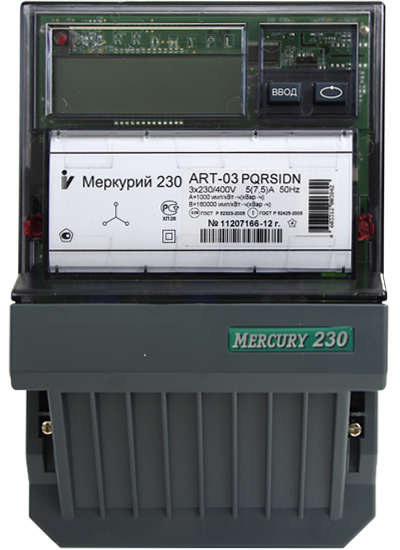
\includegraphics[scale=0.6]{img/mercury.png}
	\caption{<<Меркурий 230 ART-03>>}
\end{figure}

\newpage

\section{Протоколы}

Набор правил, позволяющий осуществлять соединение и обмен данными межджу двумя и более включёнными в сеть компьютерами, называется \textbf{сетевым протолом}.
Сами протоколы лишь описывают разные стороны одной и той же связи; взятые вместе, они образуют так называемый стек протоколов. Названия <<протокол>> и <<стек протоколов>> также указывают на программное обеспечение, которым реализуется протокол\cite{protocols}.

Распространённой системой классификации сетевых протоколов является так называемая модель OSI. В соответствии с этой моделью протоколы делятся на 7 уровней по своему назначению ~--- от физического до прикладного (см. таблицу~\ref{osi}). 

Протоколы работают друг с другом в стеке --- это означает, что протокол располагающийся на уровне выше, инкапсулируется в протокол нижнего уровня. Например, протокол UDP работает поверх протокола IP.

\begin{table}[h!]
\caption{Уровни протоколов в модели OSI}
\label{osi}
	\begin{tabular}{|c| >{\centering} m{120mm} <{\centering}|}
	\hline
	Уровень & Назначение \\
	\tabularnewline
	\hline
	Прикладной & Обеспечивает взаимодействие сети и пользователя. Уровень разрешает приложениям пользователя доступ к сетевым службам.\\
	\tabularnewline
	\hline
	Представления & Отвечает за преобразование протоколов и кодирование/декодирование данных.\\
	\tabularnewline
	\hline	
	Сеансовый & Отвечает за поддержание сеанса связи, что позволяет приложениям взаимодействовать друг с другом длительное время.\\
	\tabularnewline
	\hline
	Транспортный & Доставка данных без ошибок, потерь, дублирования и в правильной последовательности.\\
	\tabularnewline
	\hline
	Сетевой & Определение пути передачи данных. Нахождение кратчайших маршрутов.\\
	\tabularnewline
	\hline
	Канальный & Обеспечание взаимодействия сетей на физическом уровне и контроля за ошибками, которые могут возникнуть.\\
	\tabularnewline
	\hline
	Физический & Непосредственная передача потока данных через физическую среду.\\
	\tabularnewline
	\hline 
	\end{tabular}
\end{table}

\subsection{Стек протоколов TCP/IP}

\textit{Transmission Control Protocol/Internet Protocol (TCP/IP)} - это промышленный стандарт стека протоколов, разработанный для глобальных сетей\cite{tcpip}.

Этот стек протоколов был разработан до появления модели взаимодействия открытых систем. Несмотря на то, что он также имеет многоуровневую структуру, соответствие уровней стека TCP/IP уровням модели OSI весьма условно.

Работа УСПД напрямую зависит от способности поддерживать данный стек протоколов. Это объясняется следующим:
\begin{itemize}
\item Это метод получения доступа к сети Internet.
\item Это наиболее популярный и в то же время завершенный стандартный стек сетевых протоколов, имеющий многолетнюю историю
\item Все современные операционные системы поддерживают стек TCP/IP. 
\item Это устойчивая масштабируемая межплатформенная среда для приложений клиент-сервер.
\end{itemize}

Описание уровней и их назначения для стека протоколов TCP/IP можно посмотреть в таблице \ref{tcpiptable}.

\begin{table}[h!]
\caption{Стек протоколов TCP/IP}
\label{tcpiptable}
	\begin{tabular}{|c| >{\centering} m{100mm} <{\centering}|}
	\hline
	Уровень & Описание \\
	\tabularnewline
	\hline
	Прикладной & Обеспечивает взаимодействие сети и пользователя. За долгие годы использования накопилось обширное множество протоколов и сервисов прикладного уровня. Например: HTTP, FTP, SMTP, Telnet и множество других.\\
	\tabularnewline
	\hline
	Транспортный & На этом уровне функционируют два протокола. TCP и UDP. TCP обеспечивает надежную передачу сообщений между удаленными прикладными процессами за счет образования виртуальных соединений. UDP обеспечивает передачу пакетов дейтаграммным способом.\\
	\tabularnewline
	\hline
	Межсетевой & На этом уровне осуществляется передача пакетов с использованием различных транспортных технологий локальных сетей, территориальных сетей, линий специальной связи и т.п. В качестве основого протокола на этом уровне используется протокол IP. Данный протокол хорошо работает в сетях со сложной топологией.\\
	\tabularnewline
	\hline
	Физический и канальный & Этот уровень в протоколах TCP/IP не регламентируется, но поддерживает все популярные стандарты физического и канального уровня.\\
	\tabularnewline
	\hline
	\end{tabular}
\end{table}

%----------b-----------Скорее всего лишнее-------b------------%
\iffalse

\subsubsection{ARP}

\textbf{ARP} (\textit{Address Resolution Protocol}) ~--- протокол канального уровная предназначенный для установления соответствия между физическими и логическими адресами \cite{arp}.

Для определения MAC-адреса получателя по известному IP-адресу хост формирует широковещательный Ethernet-кадр, содержащий ARP-запрос (\textit{ARP-Request}). В запросе содержится MAC и IP отправителя и IP получателя. Хост, который обнаружил свой IP-адрес в поле "сетевой адрес получателя", дописывает свой MAC-адрес и отправляет ARP-ответ (\textit{ARP-Reply}). Получив искомый MAC-адрес, хост заносит его в ARP-кэш (см. таблицу \ref{arpcache}). 

\begin{table}[H]
\caption{Пример ARP-кэша}
\label{arpcache}
	\begin{tabular}{|c|c|}
	\hline
	IP-адрес & MAC-адрес\\
	\hline
	192.168.0.1 & 30:b5:c2:cd:73:90 \\
	\hline
	192.168.0.102 & f4:f5:a5:73:da:b6 \\
	\hline
	192.168.0.103 & f8:32:e4:34:e7:61 \\
	\hline
	192.168.0.101 & 00:24:21:21:26:72 \\
	\hline
	\end{tabular}
\end{table}

ARP-таблица необходима потому, что IP-адреса и MAC-адреса выбираются независимо и нет какого-либо алгоритма для преобразования одного в другой \cite{arpcitforum}.

\subsubsection{IP}

\textbf{IP} (\textit{Internet Protocol}) ~--- протокол, реализующий основу транспортных средств стека протолов TCP/IP. Является базовым элементом технологии internet, а таблица маршрутов ~--- центральная часть этого      протокола.

\paragraph{IP-адрес}

Каждый хост в IP-сети имеет свой уникальный идентификатор ~--- так называемый, \textit{IP-адрес}, который может быть получен различными способами. Он может быть присвоен статически или динамически. Длина IP-адреса --- 4 байта. Стоит отметить, что этот адрес идентифицирует точку доступа модуля IP к сетевому интерфейсу, а не всю машину целиком.

\subsubsection{ICMP}
\subsubsection{TCP}
\subsubsection{UDP}

\fi
%----------e-----------Скорее всего лишнее-------e------------%

\subsection{Универсальный синхронно-асинхронный\\ приемопередатчик (USART)}

\textbf{USART} (\textit{Universal Synchronous Asynchronous Receiver}) ~--- это модуль последовательного ввода-вывода, которые может использоваться для передачи данных с периферийными устройствами, такими как модемы, микроконтроллеры, схемы ЦАП, АЦП, терминалами, последовательными модулями расширения памяти и т.д. \cite{usart1}

USART может работать в трех режимах:
\begin{enumerate}
\item асинхронный, полный дуплекс;
\item ведомый синхронный, полудуплекс;
\item ведущий синхронный, полудуплекс;
\end{enumerate}

Модуль приемо-передатчика моежт обеспечивать полнодуплексый обмен по последовательному каналу. Скорость передачи данных может варьироваться в широких пределах. Данные посылаются последовательностями длиной от 5 до 9 битов. Также в модуле присутствует схема обеспечения повышенной помехозащищенности путем контроля и формирования бита четности.

\begin{figure}[H]
	\label{usartscheme}
	\centering
		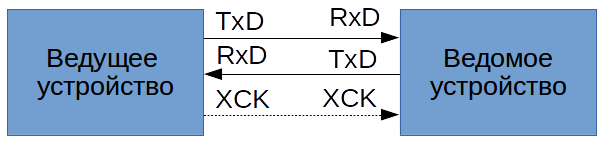
\includegraphics[scale=0.8]{img/usartscheme.png}
	\caption{Схема соединения устройств по интерфейсу USART}
\end{figure}

\textbf{Кадр} ~--- совокупность одного слова данных и сопутствующей информации \cite{usart1}. Начинается кадр со старт-бита, за которым следует младший бит слова данных. Само слово может быть длиной 5-9 битов. После 
старшего бита следует один или два стоп-бита.

\begin{figure}[H]
	\label{usartframe}
	\centering
		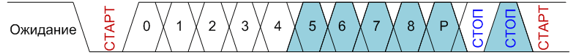
\includegraphics[scale=0.8]{img/usartframe.png}
	\caption{Кадр USART\cite{usart1}}
\end{figure}

В данной работе модуль USART будет использоваться в качестве интерфейса сетевых настроек УСПД, а также для обмена данными с датчиками и счетчиками.

\newpage

\section{Постановка задачи}

Между сервером и клиентом (УСПД) должна происходить передача данных с использованием различных сетевых стандартов. Могут комбинироваться в одном УСПД как проводные, так и беспроводные технологии передачи данных.

На транспортном уровене в стеке протоколов TCP/IP можно использовать протокол UDP, а для прикладного уровня необходимо реализовывать собственный протокол обмена данными. 

Поскольку транспортный протокол должен инкапсулироваться в протоколы нижних уровней, то для начала необходимо построить базис TCP/IP протоколов от физического до транспортного уровня. Следующие разделы будут описывать:
\begin{itemize}
\item физическое соединение УСПД по Ethernet с локальной сетью;
\item построение стека протоколов от канального (Ethernet) до транспортного (UDP);
\item описание и реализация способов конфигурации сетевых настроек УСПД;
\end{itemize}





%\chapter{ТЕХНИЧЕСКОЕ ЗАДАНИЕ}

\section{Общие положения}

\subsection{Полное наименование системы и его условное обозначение}

Полное наименование системы: Протокол обмена данными между контроллером и специализированным сервером сбора данных.

Краткое наименование: Протокол

\subsection{Наименование организации-заказчика системы}

\begin{flushleft}
\leftskip=15mm{
Заказчиком системы является ООО <<Прионежская сетевая компания>>\\
Адрес заказчика: г. Петрозаводск, ул. Новосулажгорская, 22.}
\end{flushleft}

\subsection{Плановые сроки начала и окончания работы по созданию системы}

\begin{flushleft}
\leftskip=15mm{
Плановый срок начала работ по созданию --- 01 ноября 2016 года.\\
Плановый срок окончания работ по созданию --- 15 мая 2017 года.}
\end{flushleft}

\section{Назначение и цели создания системы}

\subsection{Назначение системы}

Сделать возможным отправку данных между УСПД и сервером в сети Интернет или интранет.

\subsection{Цели создание системы}

Обеспечение отправки данных о потреблении и качества электроснабжения предприятии на сервер.


 % Скорее всего лишнее


\chapter{СХЕМА СИСТЕМЫ МОНИТОРИНГА И ВЫБОР КОМПОНЕНТОВ КОНТРОЛЛЕРА}

\section{Общая структура схемы системы мониторинга электроэнергии}

Схема дистанционного мониторинга состоит из двух частей, взаимодействующих между собой: ИИК (Информационно-измерительный канал) и ИВК (Информационно-вычислительный комплекс). ИВК можно условно разделить на два уровня - нижний и верхний. Нижний уровень уровень включает в себя:
\begin{enumerate}
	\item устройства сбора и передачи данных (УСПД);
	\item каналы связи между электросчетчиками и УСПД;
	\item контроллеры удаленного сбора данных (КУСД);
	\item коммуникационная среда и каналы связи между КУСД и серверами верхнего уровня;
\end{enumerate}

Верхний уровень включает в себя:
\begin{enumerate}
	\item серверы верхнего уровня;
	\item ПО верхнего уровня;
	\item автоматизированные рабочие места(АРМ) диспетчеров и т.д;
\end{enumerate}

В данной системе удаленного мониторинга, Устройство Сбора и Передачи Данных (УСПД) --- это счетчик электрической энергии <<Меркурий 230ART-03>>. Разрабатываемый контроллер в системе АСКУЭ выполняет функции Контроллера Удаленного Сбора Данных (КУСД). Канал связи нижнего уровня представлен шиной CAN, а коммуникационная среда между КУСД и сервером (канал связи верхнего уровня) представлена глобальной компьютерной сетью Интернет либо Локальной Вычислительной Сетью (ЛВС) на базе различных технологии (например Ethernet). К каналу связи нижнего уровня можно подключать до 240 счетчиков к одному контроллеру\cite{mercinfo1}. Удаленным серверм в АСКУЭ является компьютер на котором имеется программа, которая обеспечивает взаимодейтсвие с КУСД. В данной работе предусматривается разработка ПО только для КУСД.

Схема системы мониторинга отображена на рисунке \ref{fig:ascaepscheme}.

\begin{figure}[h!]
	\centering
		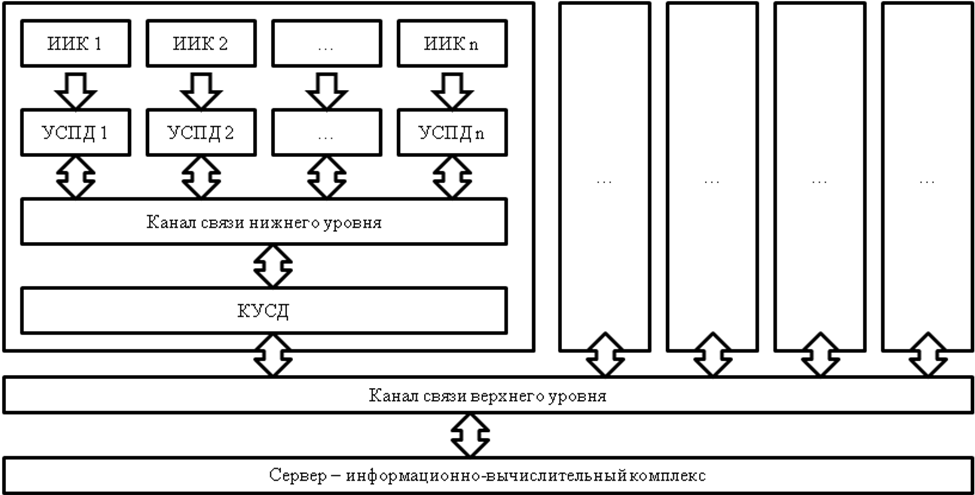
\includegraphics[scale=1.0]{img/ascaepscheme.png}
	\caption{Схема системы мониторинга электрической энергии \label{fig:ascaepscheme}}
\end{figure}

\section{Структурная схема разрабатываемого контроллера}

Связка КУСД и УСПД отображена на рисунке \ref{fig:controllerandmercury}.

\begin{figure}[h!]
	\centering
		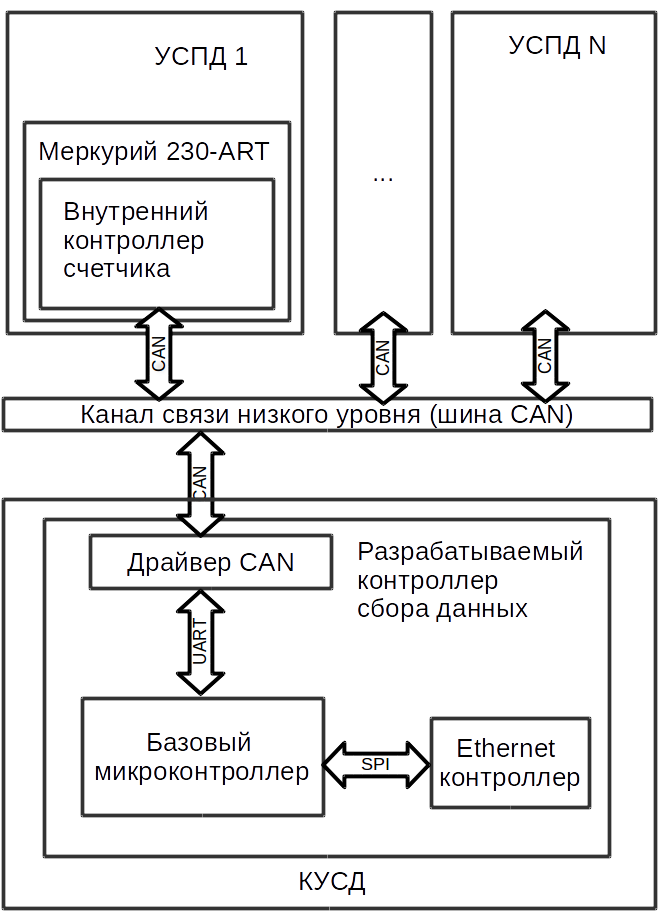
\includegraphics[scale=0.5]{img/controller_mercury.png}
	\caption{Схема системы мониторинга электрической энергии \label{fig:controllerandmercury}}
\end{figure}

Из рисунка можно выделить три основных блока КУСД:
\begin{enumerate}
	\item драйвер шины CAN;
	\item базовый микроконтроллер;
	\item Ethernet контроллер;
\end{enumerate}

\section{Программное обеспечение системы}

Программное обеспечение системы включает в себя:

\begin{enumerate}
	\item программное обеспечение КУСД и УСПД (прошивка);
	\item протокол связи между УСПД и КУСД, а также между КУСД и сервером системы;
	\item серверное программное обеспечение:
	\begin{enumerate}
		\item операционная система сервера;
		\item базы данных системы;
		\item реляционная СУБД;
		\item модуль взаимодействия с КУСПД;
	\end{enumerate}
	\item программное обеспечение пользователя системы (клиентское ПО);
\end{enumerate}

\section{Выбор компонентов контроллера}

\subsection{Базовый микроконтроллер}

Базовый микроконтроллер является основой КУСД. Перечень необходимых требований предъявляемых к микроконтроллеру:
\begin{itemize}
	\item наличие Flash-памяти программ с большим числом циклов записи;
	\item наличие энергонезависимой репрограммируемой памяти для хранения конфигурации (например EEPROM);
	\item наличие интерфейсов и портов ввода/вывода для подключения периферийных устройств:
	\begin{itemize}
		\item[•] интерфейс USART (UART) для взаимодействия с драйвером CAN, а также настроек конфигурации;
		\item[•] интерфейс SPI для сопряжения с Ethernet контроллером;
	\end{itemize}
	\item доступная цена;
	\item приемлемая для функционирования системы производительность;
	\item доступность в свободной продаже на отечественном рынке;
\end{itemize}

В соответствии с перечисленными требованиями был выбран 8-разрядный микроконтроллер ATmega328/P фирмы Atmel. Этот микроконтроллер имеет достаточную производительность, широко доступен на рынке (по состоянию на 2017 г.) по приемлемой цене и потребляет малый ток в активном режиме.

К его отличительным особенностям можно отнести\cite{atmegainfo}:
\begin{itemize}
	\item продвинутая RISC архитектура:
	\begin{itemize}
		\item[•] 131 исполняемых команд;
		\item[•] 32 рабочих регистра общего назначения;
		\item[•] полностью статический режим работы;
		\item[•] большинстов команд выполняются за один машинный такт;
		\item[•] встроенный 2-х тактовый умножитель;
	\end{itemize}
	\item износостойка и энергонезависимая память программ и данных:
	\begin{itemize}
		\item[•] 32 Кбайт репрограммируемой Flash памяти для команд;
		\item[•] 1 Кбайт EEPROM;
		\item[•] 2 Кбайт внутренней SRAM;
		\item[•] программируемый ключ для защиты прошивки;
		\item[•] срок сохранения данных: 20 лет при температуре 85 $^{\circ}$C и 100 лет при температуре 25 $^{\circ}$C;
	\end{itemize}
	\item периферийные функции:
	\begin{itemize}
		\item[•] два 8-битный таймера/счётчика с программируемым предделителем и режимом сравнения;
		\item[•] один 16-битный таймер/счетчик с программируемым предделителем, режимом сравнения и режимом захвата;
		\item[•] счётчик реального времени с программируемым генератором;
		\item[•] 6 ШИМ генераторов;
		\item[•] два 10-битных АЦП;
		\item[•] два Master/Slave SPI последовательных интерфейса;
		\item[•] один программируемый последовательный USART интерфейс;
		\item[•] программируемый Watchdog таймер с программируемым генератором;
		\item[•] встроенный аналоговый компаратор;
		\item[•] прерывания и уход из спящего режима по изменению уровня на ножке;
	\end{itemize}
	\item 23 программируемых линии ввода/вывода;
	\item напряжение питания: 1,8-5,5 В;
	\item рабочий температурный диапазон: от -40$^{\circ}$C до 105$^{\circ}$C;
	\item энергопотребление при частоте 1МГц, 1,8В, 25$^{\circ}$C:
	\begin{itemize}
		\item[•] активный режим: 0,2 мА;
		\item[•] режим энергосбережения: 0,75 мкА;
		\item[•] режим выключенного питания: 0,1 мкА;
	\end{itemize}
\end{itemize}

Для данной работы в качестве макетного образца для испытания работы сетевых протоколов будет использована готовая плата контроллера Arduino UNO R3. Внешний вид платы отображен на рисунке \ref{fig:arduino}.

\begin{figure}[h!]
	\centering
		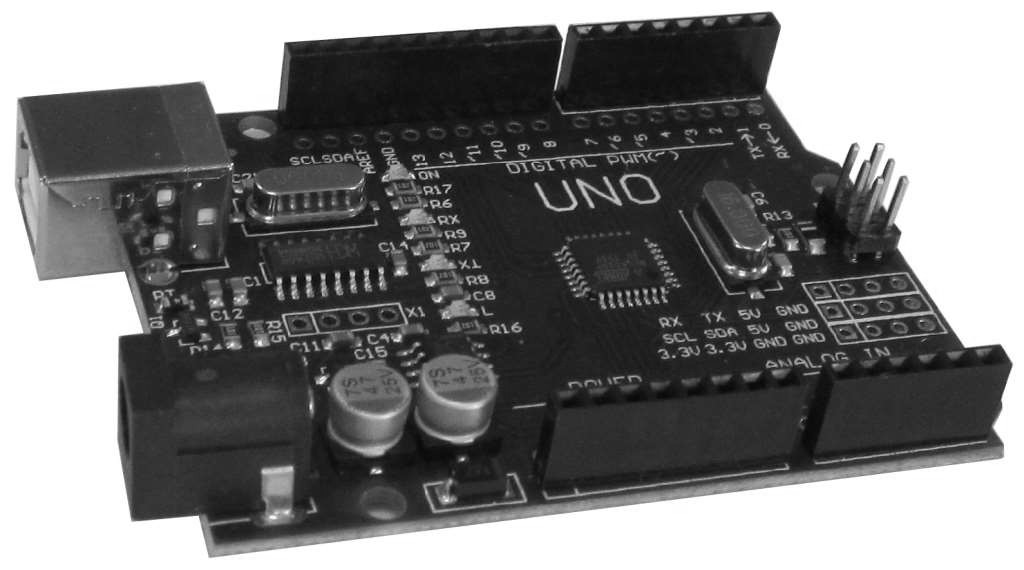
\includegraphics[scale=0.56]{img/arduino_uno_r3.jpg}
	\caption{Внешний вид платы Arduino UNO R3\label{fig:arduino}}
\end{figure}

Данная плата произведена на базе микроконтроллера ATmega328/P с тактовой частотой 16 МГц. Особенности данной платы\cite{arduino}:
\begin{itemize}
	\item питание:
	\begin{itemize}
		\item[•] может питаться как от USB подключения, так и от внешнего источника: батарейки или обычной электрической сети;
		\item[•] работает при наличии напряжения от 6 до 20 В, однако при напряжении менее 7 В работа может быть неустойчивой, а напряжение более 12 В может привести к перегреву и повреждению;
	\end{itemize}
	\item память: из 32 Кбайт Flash-памяти ATmega328/P 2 Кбайт отведено под так называемый \textit{bootloader}. Он позволяет прошивать контроллер с использованием последовательного UART интерфейса, а используя встроенный переходник USB <-> COM TTL (RS232) CH340G можно прошивать контроллер используя USB.
	\item защита USB: плата обладает предохранителем, защищающим USB-порты от перенапряжения и коротких замыканий;
	\item габариты: размер платы составляет 6,9 x 5,3 см;
\end{itemize}

\subsection{Ethernet контроллер ENC28J60}

ENC28J60 ~--- это Ethernet микроконтроллер с SPI интерфейсом. Он удовлетворяет всем спецификациям стандарта IEEE 802.3. Микросхема реализует сервисы физического уровня и MAC-подуровня канального уровня в модели OSI. На физическом уровне действует спецификация 10BASE-T PHY. Полностью совместима с 10/100/1000Base-T. Внешний вид микросхемы изображен на рисунке \ref{fig:enc28j60}.

Технические характеристики\cite{enc28j60datasheet}:
\begin{itemize}
	\item поддержка полнодуплексного и полудуплексного режима;
	\item имеет программируемую настройу расчета CRC и заполнения кадра;
	\item имеет SPI интерфейс со скоростью обмена не более 20 МГц;
	\item встроенный DMA для быстрого перемещения данных;
	\item буфер входящих пакетов является аппаратно-управляемым циклическим FIFO буфером;
	\item поддержка Unicast, Multicast и Broadcast пакетов;
	\item имеет программируемую настойку фильтрации входящих пакетов;
	\item имеет шесть источников прерываний и один вывод для внешнего прерывания;
	\item напряжения питания 3,1-3,6 В;
	\item входы толерантны к 5 В;
	\item температурный диапазон:  от -40 до +85 $^{\circ}$C.
\end{itemize}

В разрабатываемом контроллере используется готовый Ethernet модуль на базе ENC28J60. Данный модуль имеет всю необходимую для работы периферию:
\begin{itemize}
	\item <<розетка>> физического сетевого интерфейса Rj-45;
	\item кварц 25 МГц;
	\item светодиоды состояния;
	\item выводы SPI интерфейса;
	\item выводы для подключения питания 3,3/5 В;
	\item стабилизатор напряжения на 3,3 В;
\end{itemize}

Внешний вид модуля изображен на рисунке \ref{fig:ethcontroller}.

\begin{figure}[h!]
	\centering
		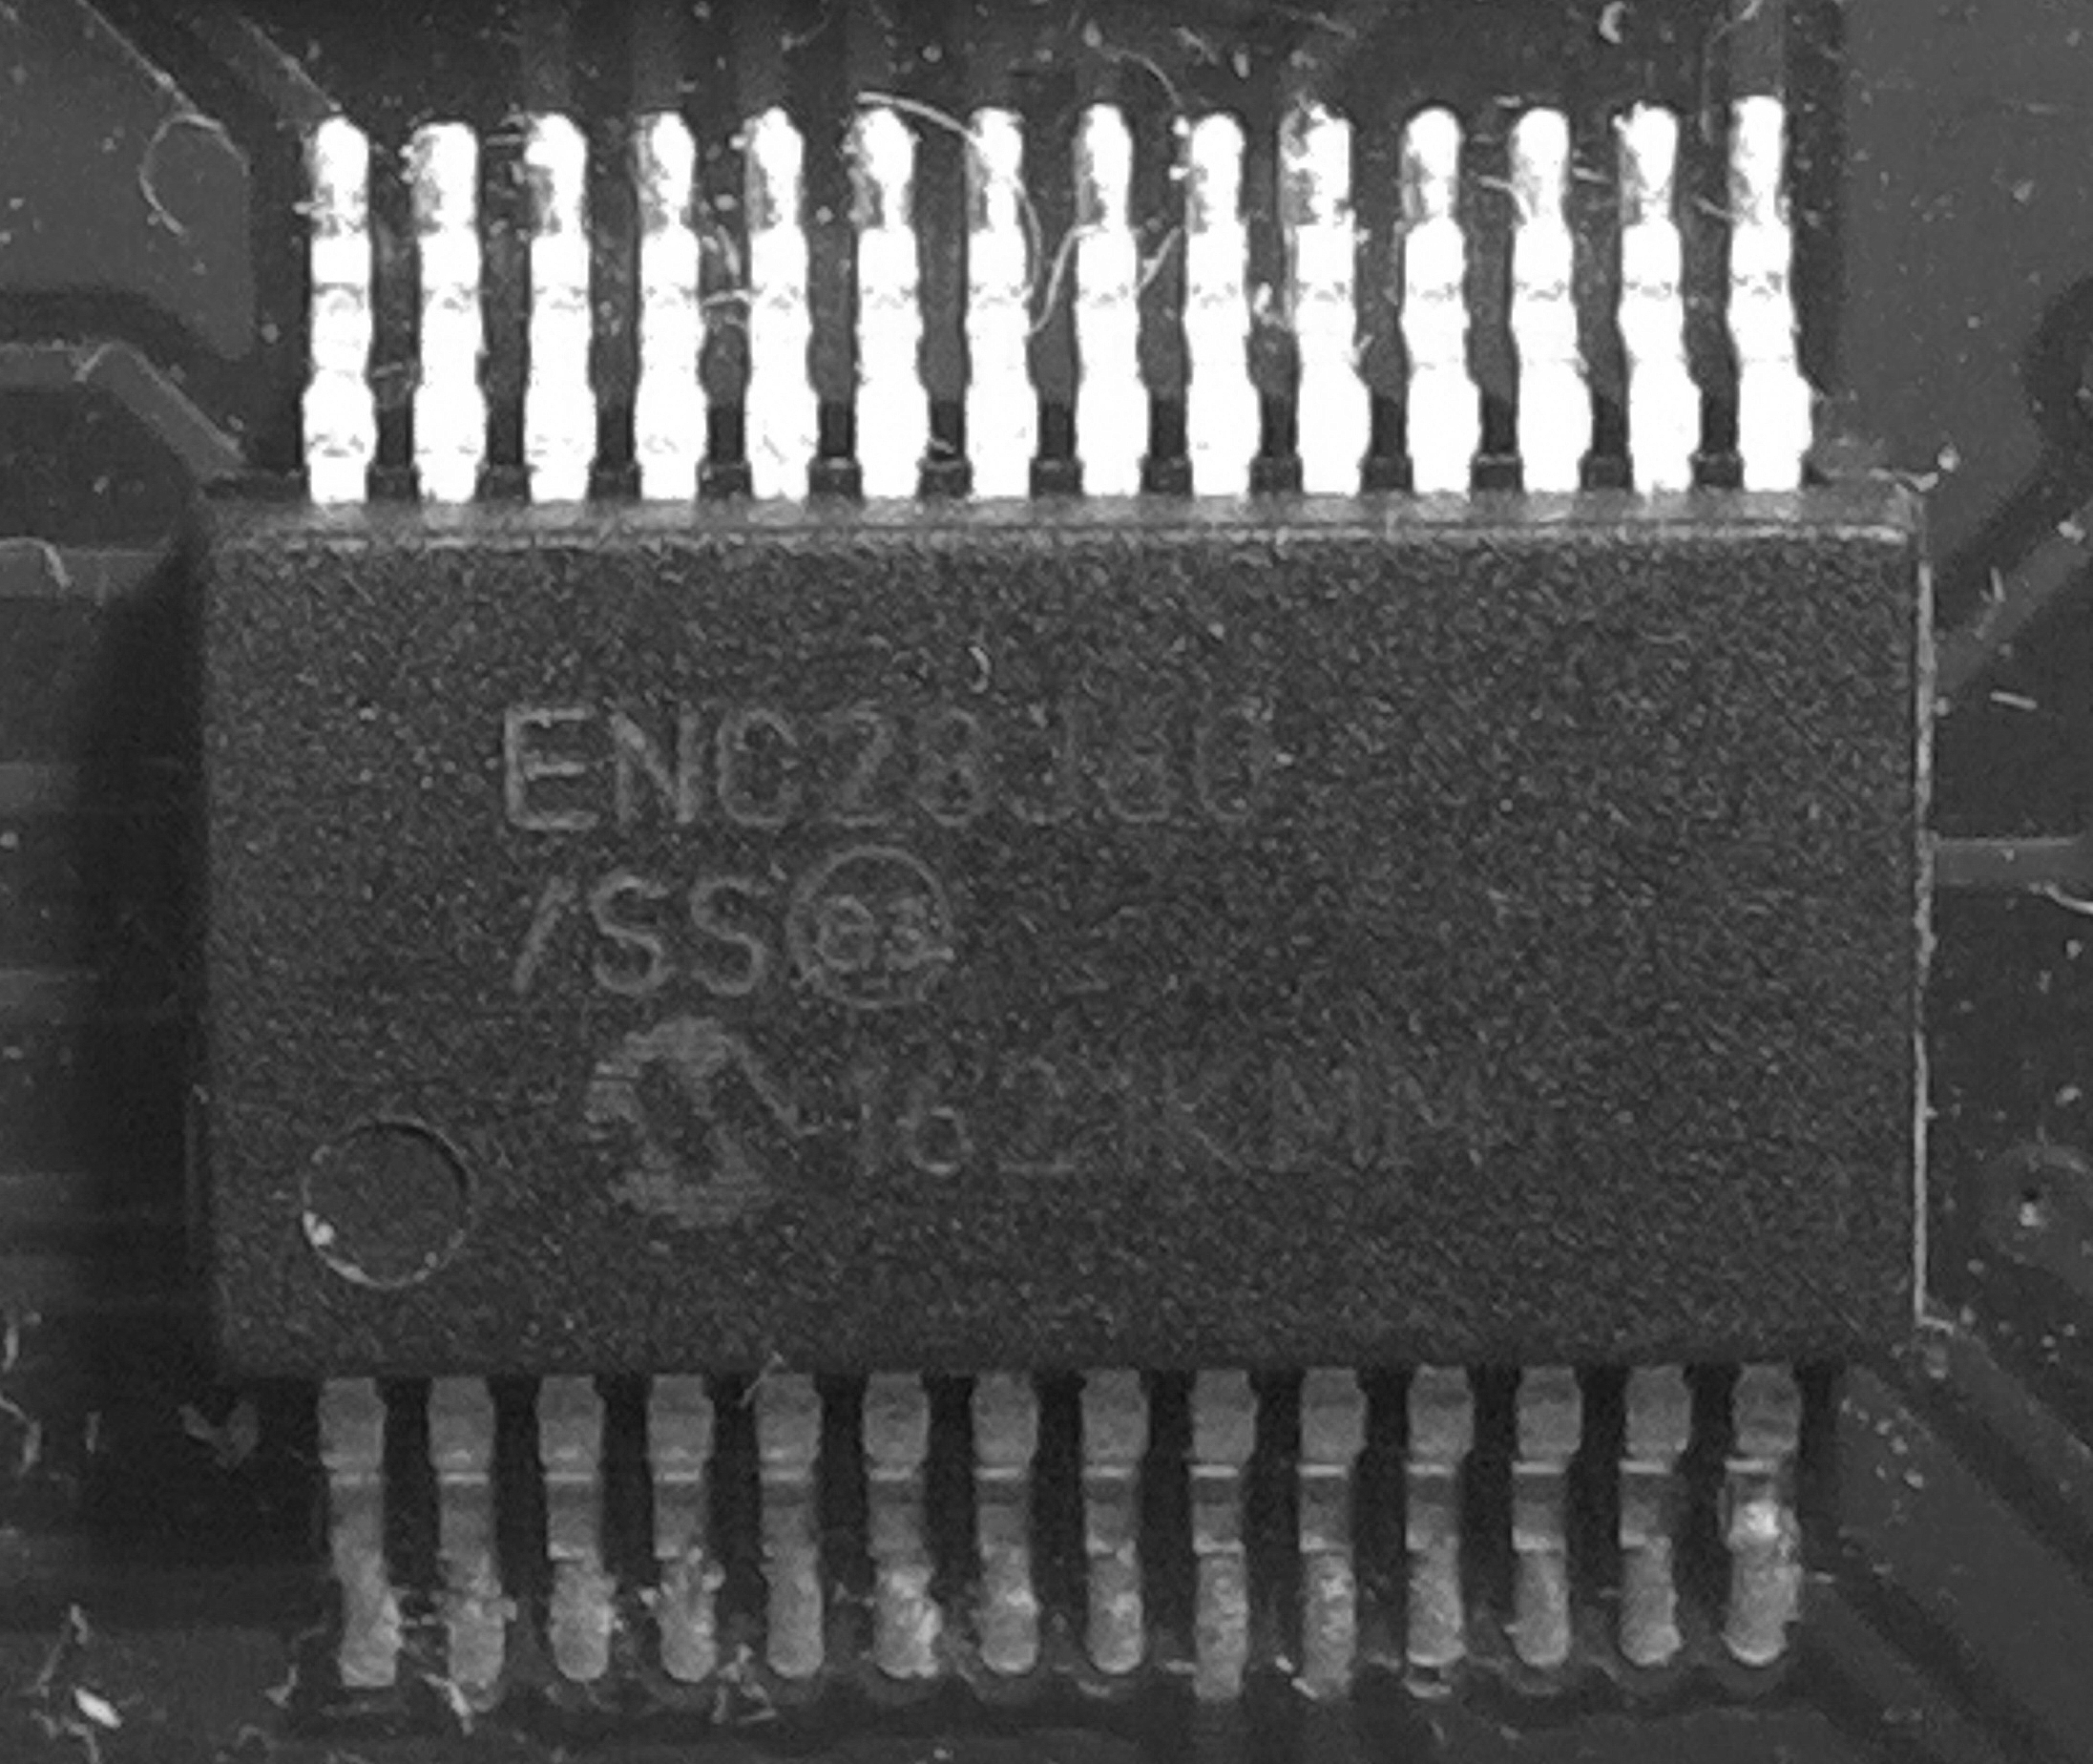
\includegraphics[scale=0.09]{img/enc28j60.png}
		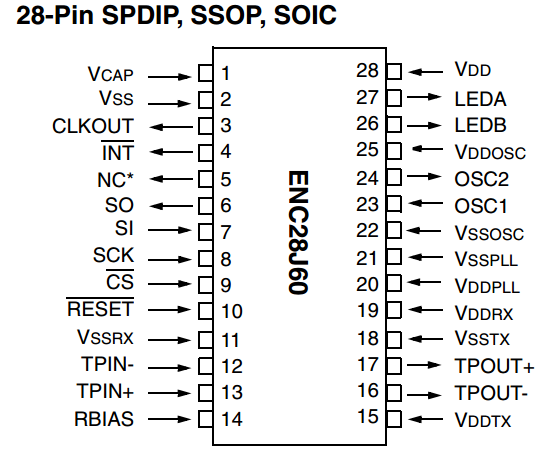
\includegraphics[scale=0.36]{img/enc28j60io.png}
	\caption{Внешний вид микросхемы ENC28J60 и расположение выводов\label{fig:enc28j60}}
\end{figure}


\begin{figure}[h!]
	\centering
		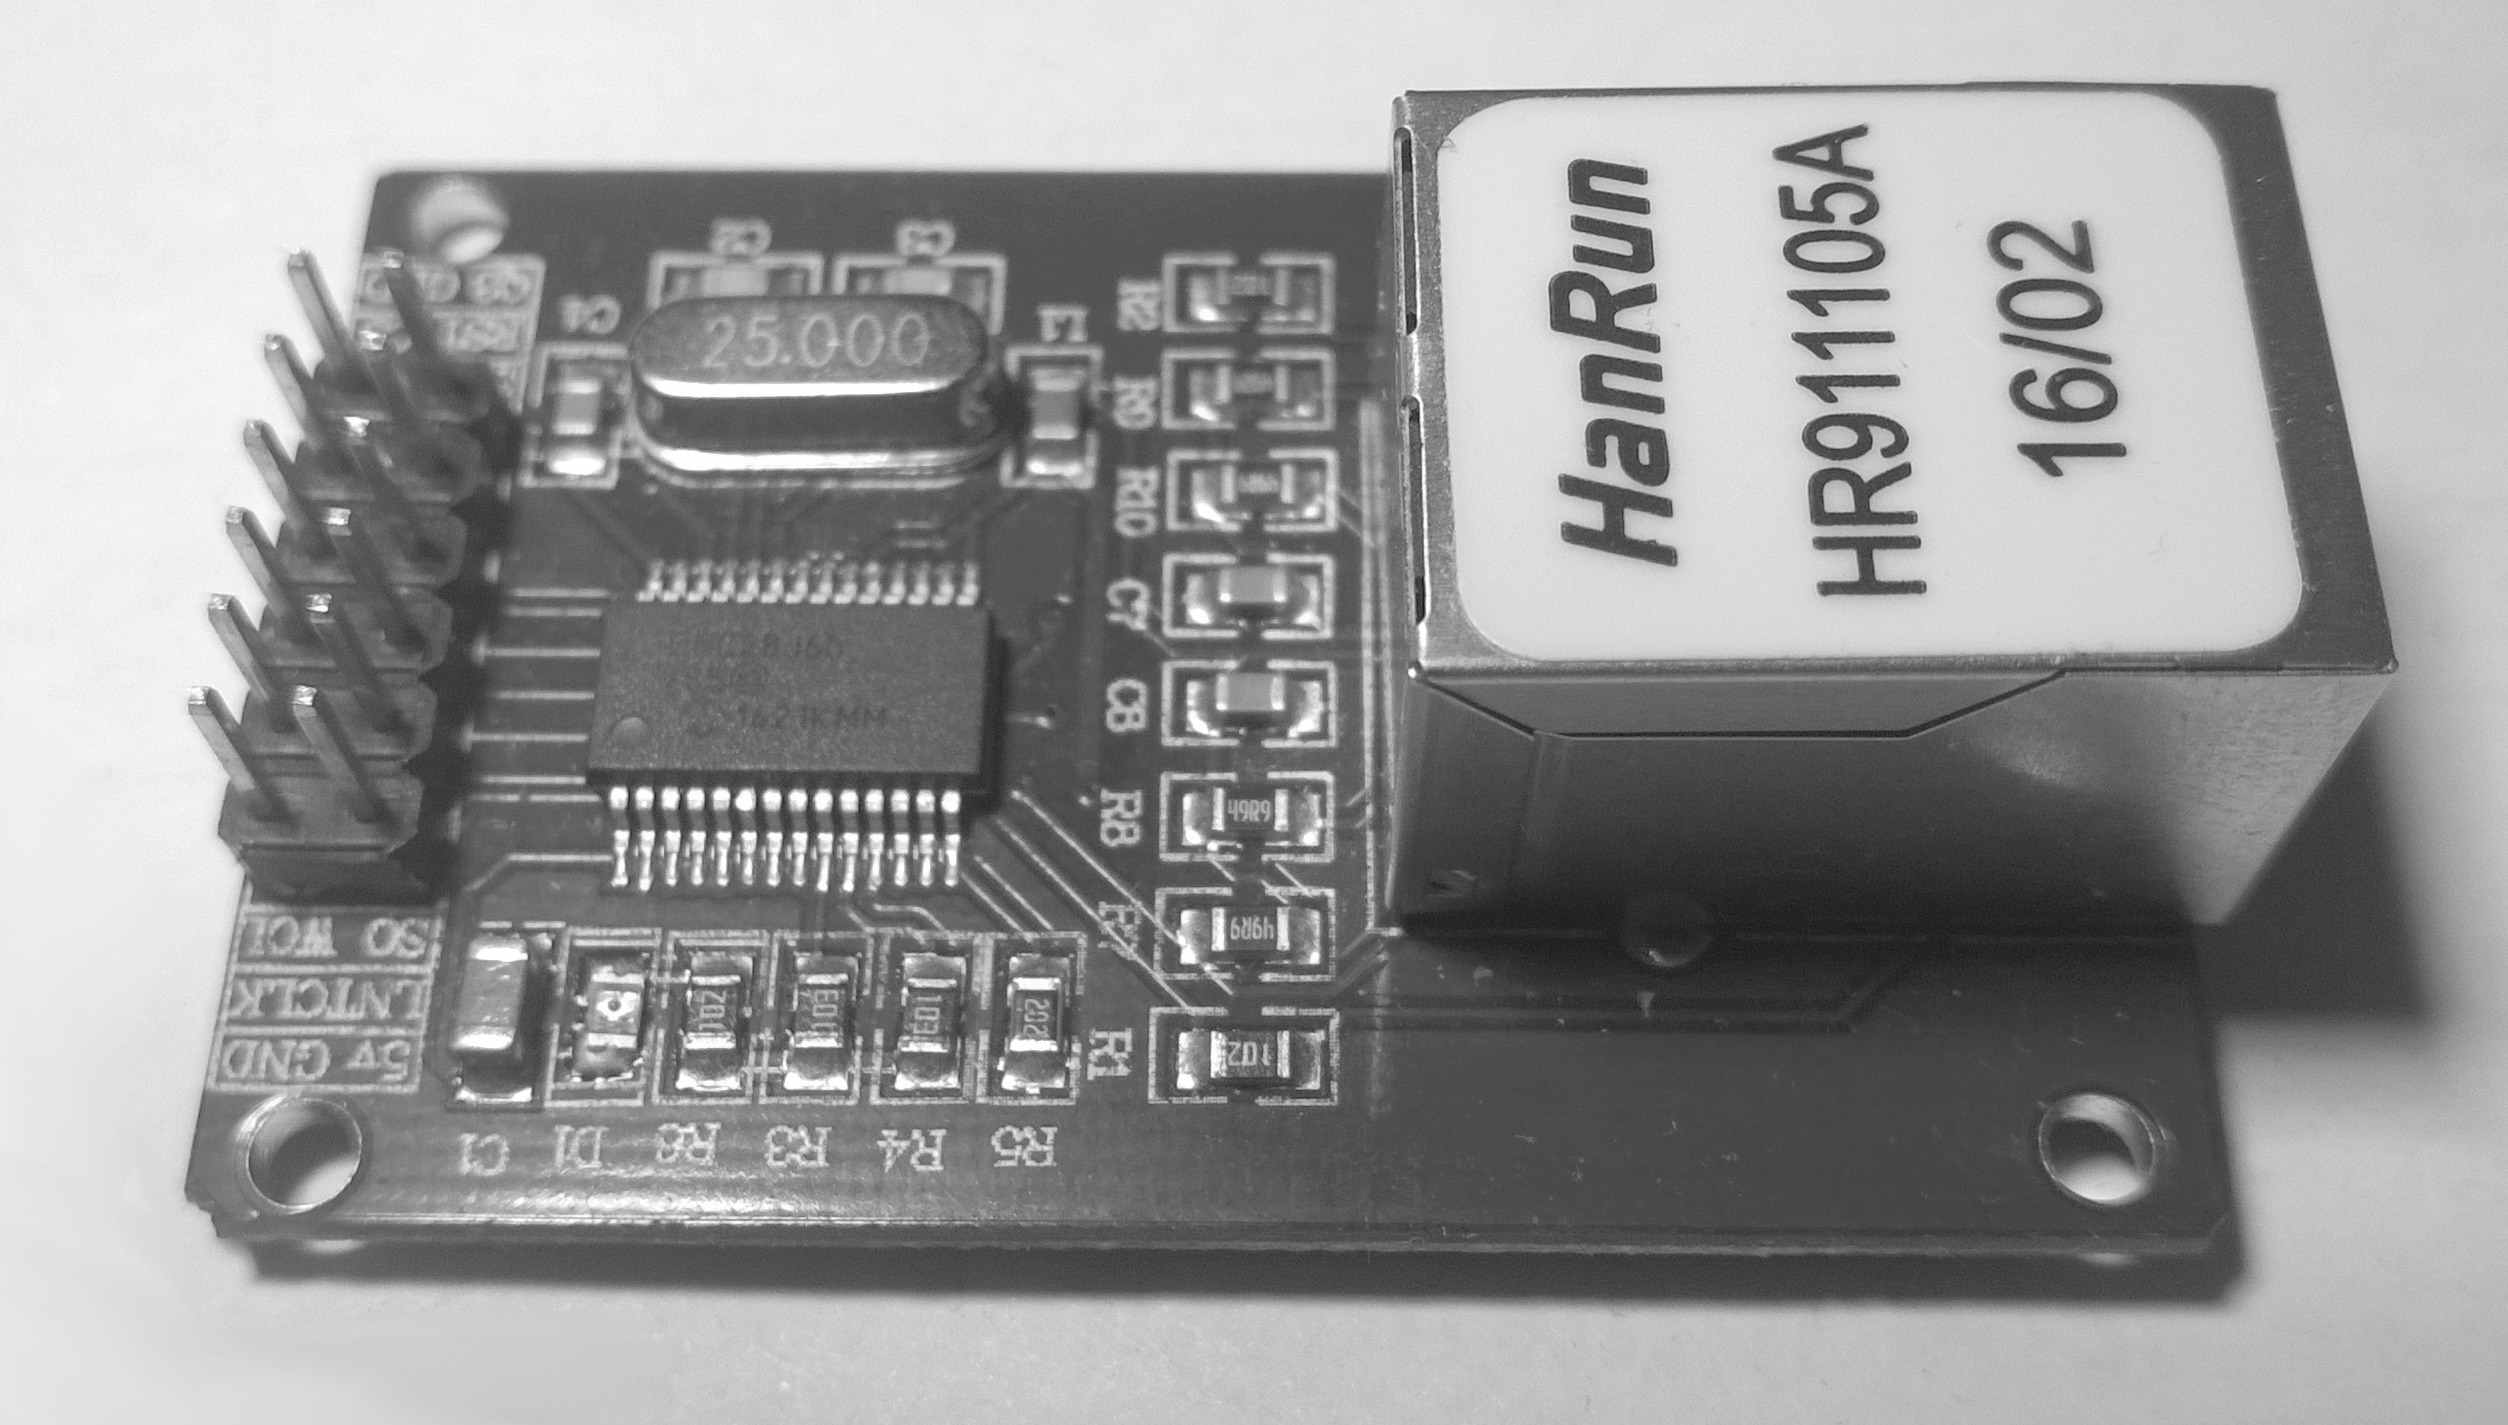
\includegraphics[scale=0.1]{img/ethcontroller.png}
		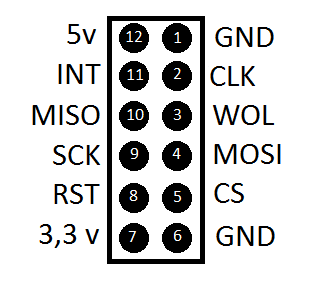
\includegraphics[scale=0.5]{img/ethpins.png}
	\caption{Внешний вид модуля и расположение выводов для подключения к КУСД\label{fig:ethcontroller}}
\end{figure}





\chapter{РЕАЛИЗАЦИЯ}

\section{Программное обеспечение КУСД}

Работа КУСД, как было сказано ранее (стр. \pageref{reasonofwork}), полностью зависит от поддержки стека сетевых протоколов TCP/IP. Следовательно, основная часть данной работы направлена на создание программного обеспечения, реализующего поддержку стека сетевых протоколов.

В качестве инструмента реализации программного обеспечения использовался домашний компьютер с ОС Linux Ubuntu 16.04, на котором было установлен следующее ПО:
 \begin{itemize}
	\item набор GNU AVR Toolchain версии 4.9.2, в который входит\cite{avrtoolchain}:
	\begin{itemize}
		\item[•] компилятор avr-gcc, для комплиляции исходного кода на языке С/С++ в машинный язык микроконтроллеров семейства AVR;
		\item[•] набор ассемблера и компоновщика avr-binutils;
		\item[•] avr-libc --- подмножество стандартной библиотеки С с некоторыми специфичными для AVR функциями;
		\item[•] avr-gdb --- отладчик;
		\item[•] avrdude --- программа для загрузки/выгрузки/управления памятью программ и данных на МК AVR;
	\end{itemize}
	\item интегрированная среда разработки Elcipse версии 3.8.1 с плагином для разработки программ на МК AVR;
\end{itemize}

\section{Работа с Ethernet-контроллером}

Первоначально требовалось обеспечить передачу данных между Ethernet-контроллером и микроконтроллером ATmega328/P по шине SPI. Опираясь на таблицу \ref{spitabl}, а также на расположение выводов контроллера enc28j60 (рисунок \ref{fig:ethcontroller}), микроконтроллер был подключен к Ethernet-контроллеру. Соответсвие выходам микроконтроллера ATmega328/P и входам Ethernet-контроллера описано в таблице \ref{connection}. Стоит отметить что хоть Ethernet-контроллер в основном оперирует напряжением 3,3 В, на вход питания можно подавать 5 В и выше, поскольку на плате присутствует стабилизатор напряжения AMS1117\cite{voltageregulator}. После подключение убеждаемся в том, что на плату Ethernet-контроллера поступает питание по свечению светодида D1. 

\begin{table}[h!]
\caption{Соответствие выходам ATmega328/P и входам Ethernet-контроллера в данной работе}
\label{connection}
	\begin{tabular}{|p{40mm}|p{40mm}|p{40mm}|}
\hline
	Наименование соединения & Выход на ATmega328/P & Вход на Ethernet-контроллере \\
\hline
		MOSI & PB3 & MOSI (4)\\
\hline
		MISO & PB4 & MISO(10)\\
\hline
		SCLK & PB5 & SCK(9)\\
\hline
		SS & PB2 & CS (5)\\
\hline
\end{tabular}
\end{table}

Для взаимодействия с Ethernet-котроллером была написана библиотека на языке Си. Здесь и далее форматы заголовков различных протоколов будут описываться структурами данных на языке Си. Заранее определим используемые типы и определения:
\begin{itemize}
	\item типы:
	\begin{itemize}
		\item[•] \textit{uint8\_t} --- безнаковое целое число, 8 бит;
		\item[•] \textit{uint16\_t} --- безнаковое целое число, 16 бит;
		\item[•] \textit{uint32\_t} --- безнаковое целое число, 32 бита;
	\end{itemize}
	\item определения:
	\begin{itemize}
		\item[•] \textit{htons(a)} --- макрос, обеспечивающий перевод порядка байтов, принятого у данного хоста, к сетевому (2 байта);
		\item[•] \textit{htonl(a)} --- макрос, обеспечивающий перевод порядка байтов, принятого у данного хоста, к сетевому (4 байта);
		\item[•] \textit{ntohs(a)} --- макрос, обеспечивающий перевод от сетевого порядка байтов до порядка, принятого у данного хоста (2 байта);
		\item[•] \textit{ntohl(a)} --- макрос, обеспечивающий перевод от сетевого порядка байтов до порядка, принятого у данного хоста (4 байта);
	\end{itemize}
\end{itemize}

Основной интерфейс данной библиотеки представлен в листинге \ref{lst:enc28j60header}. 

{\small{\lstinputlisting[language=C, caption=Интерфейс для взаимодействия с ENC28J60 по шине SPI\label{lst:enc28j60header}, inputencoding=cp1251, linerange={12-33}]{./src/enc28j60.h}}}

Алгоритм работы с Ethernet-контроллером следующий:
\begin{enumerate}
	\item настраиваем работу по шине SPI: 
		\begin{itemize}
			\item конфигурируем выходы микроконтроллера CS, MOSI, SCK на запись, а MISO на чтение;
			\item устанавливаем режим работы SPI интерфейса ATmega328/P как ``Мастер'';
			\item выставляем скорость работы шины SPI на максимальную;
			\item используем SPI режим 0 (CPOL=0, CPHA=0);
		\end{itemize}
	\item инициализируем ENC28J60:
		\begin{itemize}
			\item делаем ``мягкий сброс'' микросхемы;
			\item устанавливаем размер FIFO для приема данных (ERXST, ERXND), инициализируем указатель для чтения данных из FIFO (ERXRDPT);
			\item конфигурируем MAC: включаем аппаратное управление потоком, автоматическое выравнивание до 60 байт, автоматическое добавление контрольной суммы, устанавливаем MAC-адрес в регистрах MAADR;
			\item настраиваем PHY: устанавливаем дуплексный режим, настраиваем индикаторные светодиоды, отключаем loopback;
			\item разрешаем прием пакетов;
		\end{itemize}
	\item принимаем и отправляем пакеты;
\end{enumerate}

После того, как мы получили возможность обмениваться сырыми данными с другими Ethernet-устройствами, осталось написать протоколы канального, сетевого и транспортного уровня.

\section{Реализация протоколов стека TCP/IP}

\subsection{Ethernet}

Заголовки протокола Ethernet представлены в листинге \ref{lst:ethernethead}. 

{\small{\lstinputlisting[language=C, caption=Определение полей и заголовков для манипулирования Ethernet-кадрами\label{lst:ethernethead}, inputencoding=cp1251, linerange={13-13, 41-49}]{./src/lan.h}}}

Далее требовалось реализовать поддержку протокола сетевого уровня IP, что бы успешно взаимодействовать с другими хостами в сети, построенной на базе стека протоколов TCP/IP.

\subsection{IP}

\textbf{IP} (\textit{Internet Protocol}) ~--- протокол, реализующий основу транспортных средств стека протолов TCP/IP. Является базовым элементом технологии Internet, а таблица маршрутов ~--- центральная часть этого протокола. Каждый хост в IP-сети имеет свой уникальный идентификатор ~--- так называемый, \textit{IP-адрес}, который может быть получен различными способами. Он может быть присвоен статически или динамически. Длина IP-адреса --- 4 байта. Стоит отметить, что этот адрес идентифицирует точку доступа модуля IP к сетевому интерфейсу, а не всю машину целиком.

Стоит подробнее рассмотреть таблицу машрутизации, которая хранится в КУСД. Данная таблица описывает соответсвие между адресами назначения и интерфейсами, через которые следует отправить пакет данных до следующего маршрутизатора \cite{ip}. Она обычно содержит:
\begin{itemize}
	\item[•] \textit{Destination} --- адрес сети или узла назначения, либо указание, что маршрут является маршрутом по умолчанию;
	\item[•] \textit{Netmask} --- маска сети назначения;
	\item[•] \textit{Gateway}, или \textit{Next Hop} --- следующий маршрутизатор;
	\item[•] \textit{Interface} --- интерфейс (численный или символьный идентификатор устройства);
	\item[•] \textit{Metric} --- число, соответствующее предпочтительности маршрута (чем число меньше, тем более предпочтителен маршрут);
\end{itemize}

Поскольку в данной работе имеется только макет КУСД и нет цели использовать все возможности таблицы маршрутизации, используется информация о маске подсети в которой находится КУСД, его IP-адрес и стандартный маршрутизатор. Заголовки протокола IP и таблица маршрутизации представлены в листинге \ref{lst:iphead}.

{\small{\lstinputlisting[language=C, caption=Определение полей и заголовков для манипулирования IP-датаграммами\, таблица маршрутизации\label{lst:iphead}, inputencoding=cp1251, linerange={14-18, 82-98}]{./src/lan.h}}}

\subsection{ARP}

После того как определен и реализован некоторый базис, позволяющий передавать пакеты в локальной сети, небходимо связать канальный и сетевые уровни протоколом \textbf{ARP} (\textit{Address Resolution Protocol})\cite{arp}. Это необходимо поскольку не существует другого явного алгоритма преобразования IP-адрес в MAC-адреса\cite{arpcitforum}.

Рассмотрим процедуру преобразования адресов при отправлении сообщения. Пусть один хост отправляет сообщение другому. Прикладной программе IP-адрес места назначения обычно известен. Для определения MAC-адреса просматривается ARP-таблица. Если для требуемого IP-адреса в ней присутствует MAC-адрес, то формируется и посылается пакет по соответствующему адресу. Если же с помощью APR-таблицы не удается преобразовать адрес, то выполняется следующее:
\begin{itemize}
	\item всем хостам в сети посылается пакет с ARP-запросом (с широковещательным MAC-адресом);
	\item исходящий IP-пакет ставится в очередь;
\end{itemize}

Каждый хост, принявший ARP-запрос, в своем ARP-модуле сравнивает собственный IP-адрес с IP-адресом в запросе. Если IP-адрес совпал, то прямо по MAC-адресу отправителя запроса посылается ответ, содержащий как IP-адрес ответившей машины, так и её MAC-адрес. Далее ответ принимается и заносится в ARP-таблицу, после чего отправляются все IP-пакеты которые были занесены в очередь на отправку к данному хосту. В противном случае (такой машины в сети нет) все IP-адреса по данному адресу отбрасываются. Пример ARP-таблицы отображен в таблице \ref{arptable}.

\begin{table}[h!]
\caption{Пример упрощенной ARP-таблицы}
\label{arptable}
	\begin{tabular}{|c|c|}
	\hline
	IP-адрес & MAC-адрес\\
	\hline
	192.168.0.1 & 30:b5:c2:cd:73:90 \\
	\hline
	192.168.0.102 & f4:f5:a5:73:da:b6 \\
	\hline
	192.168.0.103 & f8:32:e4:34:e7:61 \\
	\hline
	192.168.0.101 & 00:24:21:21:26:72 \\
	\hline
	\end{tabular}
\end{table}

Заголовки протокола ARP представлены в листинге \ref{lst:arphead}.

{\small{\lstinputlisting[language=C, caption=Определение полей и заголовков для протокола ARP\label{lst:arphead}, inputencoding=cp1251, linerange={20-20, 56-78}]{./src/lan.h}}}

\subsection{ICMP}

Для тестирования работоспособности сетевого интерфейса (и вообще КУСД) не будет лишним реализовать поддержку протокола \textbf{ICMP}, а именно ICMP Echo запросы и ответы. Сам протокол ICMP служит для диагностики состояния сети. Echo-запросы имеют следующие поля:
\begin{enumerate}
	\item тип пакета: запрос (8) или ответ (0);
	\item код пакета --- 0 для Echo-запроса и ответа;
	\item контрольная сумма заголовка рассчитывается также, как и для заголовка IP-пакета;
	\item остальные поля устанавливаются на усмотрение хоста. Ответ должен содержать те же значения;
\end{enumerate}

Заголовки протокола ICMP (для Echo-запросов) представлены в листинге \ref{lst:icmpecho}.

{\small{\lstinputlisting[language=C, caption=Определение полей и заголовков для ICMP Echo запросов\label{lst:icmpecho}, inputencoding=cp1251, linerange={106-119}]{./src/lan.h}}}

Убедимся, что контроллер отвечает на Echo-запросы, отправив по его IP-адресу Echo-запрос. При этом, контроллер будет находится в домашней локальной сети по IP-адресу 192.168.0.140 и маской подсети 255.255.255.0. Отправим несколько Echo-запросов используя утилиту \textbf{ping} на одном из хостов в локальной сети (рисунок \ref{fig:echo-req}). При этом, будут считываться сообщения приходящие от самого контроллера по протоколу USART на домашний компьютер (рисунок \ref{fig:echo-reply-log}).

\begin{figure}[h!]
	\centering
		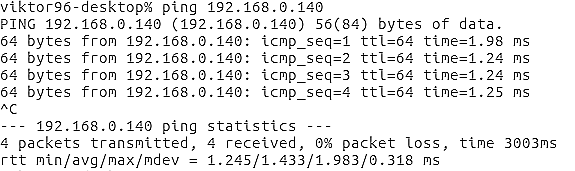
\includegraphics[scale=0.8]{img/icmp-req.png}
	\caption{Отправка Echo-запросов к КУСД\label{fig:echo-req}}
\end{figure}

\begin{figure}[h!]
	\centering
		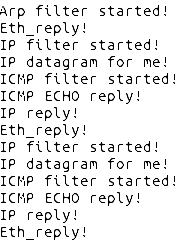
\includegraphics[scale=0.7]{img/echo-reply-log.png}
	\caption{Подтверждения о доставке Echo-запросов и ответа на них\label{fig:echo-reply-log}}
\end{figure}

Данные отладочные сообщают о том, что принятыей пакет прошел стадии обработки Ethernet фильтра, где контроллер распознал свой MAC-адрес, следом IP фильтра, где контроллер распознал свой IP-адрес, далее ICMP фильтра, в котором был распознан код и типа сообщения (код Echo-запроса, тип --- запрос). Далее последовал Echo-ответ, который собирался последовательно от уровня ICMP до Ethernet и был послан в сеть.

Как видно из рисунка \ref{fig:echo-req} по тому, что на все запросы были посланы ответы, стек протоколов от Ethernet до ICMP на данном контроллере работоспособен.

\subsection{UDP}

\textbf{UDP} (\textit{User Datagram Protocol}) ~--- простейший протокол транспортного уровня. Используется для отсылки данных некритичных к потере информации приложений. Также UDP используется для рассылки групповых IP датаграмм. Формат UDP заголовка представлен в листинге \ref{lst:udphead}.

{\small{\lstinputlisting[language=C, caption=Определение UDP заголовка\label{lst:udphead}, inputencoding=cp1251, linerange={125-131}]{./src/lan.h}}}

\section{Настройка и взаимодействие КУСД через USART}

В процессе первого монтажа и наладки работы КУСД требуется осуществить настройку его сетевых параметров. Всё это необходимо делать в условиях минимального количества дополнительных инструментов, которые должны быть у монтажника в момент установки и наладки. Было принято решение использовать интерфейс USART для настройки сетевых параметров, а также тестирования работы КУСД. Использование такого распространенного интерфейса позволяет получить доступ к настройкам КУСД, не используя узко-специализированное программное обеспечение. Для повышения безопасности можно снабдить КУСД закрытым паролем, который будет известен только той организации, которой предоставляется информация о состоянии сети. Верификация пароля будет происходить на начальном этапе установления сеанса связи по USART.

Особенностью данного интерфейса взаимодействия является то, он --- текстовый. Текстовый способ взаимодействия, против бинарного, был выбран по следующим причинам:
\begin{enumerate}
	\item это человеко-читаемый интерфейс, а это значит, что он будет понятен;
	\item не требует специальных средств расшифровки бинарных данных;
	\item позволяет использовать любой текстовый USART терминал, что расширяет круг устройств которые могут считывать и посылать на КУСД данные;
\end{enumerate}

Однако такой выбор имеет и недостатки:
\begin{enumerate}
	\item память программ КУСД должна быть достаточно большой (от 8 Кбайт и более) для поддержки текстового интерфейса;
	\item такому интерфейсу свойственны все недостатки текстовых компьютерных интерфейсов: переполнение буфера, опечатки, медлительность работы;
\end{enumerate}

Была написана библиотека на языке Си, для микроконтроллера ATmega328/P, реализующая прием и отправку данных по USART. Её интерфейс отображен в листинге \ref{lst:usartif}.

{\small{\lstinputlisting[language=C, caption=Интерфейс взаимодействия с USART\label{lst:usartif}, inputencoding=cp1251, linerange={17-33}]{./src/usart.h}}}

Далее была написана программа (см. листинг \ref{lst:main}), которая выполняет активный прием и передачу пакетов, а также способная, в режиме реального времени, изменять сетевые конфигурации КУСД. Логику работы программы лучше всего описывает модель кончного автомата. Всего имеется 4 состояния:
\begin{itemize}
	\item прослушка порта;
	\item отображение конфигурации;
	\item настройка конфигурации;
	\item командный режим;
\end{itemize}

Находясь в состоянии "прослушка порта", КУСД принимает все пакеты, которые приходят извне, а также отправляет данные о энергопотреблении удаленному серверу сбора данных. При этом если это ICMP или ARP запросы, то на них немедленно высылаются соответствующие ответы. В состоянии "отображение конфигурации" КУСД отправляет данные о своих сетевых настройках. В режиме настройка конфигурации возможно изменение сетевых параметров контроллера. В командном режиме осуществляется как прием пакетов, так и выполнение некоторого перечня команд, например отправки пакета на определенный адрес (для тестирования). Переход из одного состояния в другой происходит по, приходящим из интерфейса USART, однобайтовым текстовым командам (например символ 'h' - команда для отображения подсказки). Для взаимодействия с контроллером была использована утилита \textbf{picocom v1.7}, она реализует текстовый интерфейс взаимодействия по протоколу USART и другим. Текстовый интерфейс настройки КУСД отображен ниже:

\begin{verbatim}
picocom v1.7

port is        : /dev/ttyUSB0
flowcontrol    : none
baudrate is    : 9600
parity is      : none
databits are   : 8
escape is      : C-a
local echo is  : yes
noinit is      : no
noreset is     : no
nolock is      : no
send_cmd is    : sz -vv
receive_cmd is : rz -vv
imap is        : lfcrlf,
omap is        : 
emap is        : crcrlf,delbs,

Terminal ready
USART: Setup success!
End of initialization enc28j60

STATE: Polling

To start work:
s - view interface settings
c - configure interface settings
d - enter to command mode
l - enable/disable logger
h - help
%>
\end{verbatim}

Рассмотрим установленные текущие сетевые конфигурации, отправив символ-команду 's' (settings):
\begin{verbatim}
%> s
STATE: View

MAC = 0x0013 0x3301 0x2548 
IP = 192.168.0.140
Subnet mask = 255.255.255.0
Default gateway = 192.168.0.1
Server IP = 192.168.0.104

STATE: Polling
\end{verbatim}

Можно увидеть следующие сетевые параметры: MAC-адрес устройства, IP-адрес устройства, маска подсети, шлюз по умолчанию, адрес сервера сбора данных. Рассмотрим, процесс изменения настроек. Допустим нужно изменить IP-адрес сервера на 192.168.0.107. Отправляем символ-команду 'c':

\begin{verbatim}
%> c
STATE: Configure

MAC = 0x0013 0x3301 0x2548 
IP = 192.168.0.140
Subnet mask = 255.255.255.0
Default gateway = 192.168.0.1
Server IP = 192.168.0.104

tap 'q' to quit

change:
i - IP
m - mask
d - default
s - server IP
\end{verbatim}

На выбор предлагается изменить один из параметров. Выберем \textit{server IP}.

\begin{verbatim}
s
Enter address in x.x.x.xs format (s - stop):
\end{verbatim}

Вводим IP-адрес в требуемом формате:

\begin{verbatim}
192.168.0.107s
Configuration successfully seted

MAC = 0x0013 0x3301 0x2548 
IP = 192.168.0.140
Subnet mask = 255.255.255.0
Default gateway = 192.168.0.1
Server IP = 192.168.0.107

tap 'q' to quit

change:
i - IP
m - mask
d - default
s - server IP
\end{verbatim}

КУСД информирует об успешном изменении параметров сети, печатает новые конфигурации и предлагает выбрать следующий вариант настроек. При отправке команды 'q', КУСД вернется в режим приема и передачи пакетов.

Далее отправим тестовый UDP-пакет с сообщением ``Hello! I'm MCU!'' на ``удаленный сервер'' (функция send\_udp\_test в главной программе). ``Удаленным сервером будет'' один из компьютеров в локальной сети. Для этого перейдем в командный режим:

\begin{verbatim}
To start work:
s - view interface settings
c - configure interface settings
d - enter to command mode
l - enable/disable logger
h - help
%> d
STATE: Command mode

tap 'q' to quit

s - send test udp packet to server
\end{verbatim}

И отправим команду 's', которая заставит КУСД выслать тестовый пакет по адресу 192.168.0.107:

\begin{verbatim}
s
Test packet was sent

tap 'q' to quit

s - send test udp packet to server
\end{verbatim}

Видим, что пакет был отправлен. На другом хосте в этот момент работал сниффер (сетевой анализатор трафика) \textbf{tshark}.

\begin{verbatim}
# ---------- На хосте с IP-адресом 192.168.0.107 --------------------
# Перехват приходящих от КУСД пакетов
viktor96-desktop% tshark -f "src host 192.168.0.140" -w dump.pcap 
viktor96-desktop% tshark -r dump.pcap -T fields -e data | perl -e \ 
pipe>  '$hex = (<>)[1]; while($hex =~/(.{2})/sg) {print chr(hex($1))}'
Hello! I'm MCU!		# <-- Сообщение, посланное КУСД поверх UDP
\end{verbatim}

Сообщение было успешно принято, а его содержимое распознано.

На будущее запланирована поддержка протокола DHCP для динамической настройки сетевых параметров, а также написание программного обеспечения для удаленного изменения сетевых параметров (собственный протокол поверх UDP). Дополнительно к этому будут рассмотрены вопросы считывания данных от счетчиков и ввод КУСД в режим пониженного энергопотребления.


%-------------------конец основной части------------------------------------%

\backmatter %% Здесь заканчивается нумерованная часть документа и начинаются заключение и ссылки


\Conclusion

Был проведен обзор системы АСКУЭ. Описана клиентская часть данной системы. Описаны технологии которые могут активно применятся при разработке КУСД, обеспечивая гибкость, надежность и расширяемость данной реализации.

Написано тестовое ПО для проверки и отладки некоторых сетевых возможностей КУСД. Рассмотрены различные способы конфигурирования сетевых настроек контроллера. Планируется использование беспроводных технологии передачи данных в будущем, а также увеличение количества поддерживаемых сетевых протоколов.


%% Альтернативное оформление библиографического списка:
\begin{thebibliography}{99}

\bibitem{qualitymonitor} Монитор качества электроэнергии. [Электронный ресурс] /  Режим доступа: http://fidercom.ru/pribory-uchyota-elektroenergii/monitoring-kachestva-\\elektroenergii.html. --- (Дата последнего обращения: 13.05.2017).

\bibitem{ascaepinfo} Автоматизированная система коммерческого учета электроэнергии (АСКУЭ). / Н.М. Гришагина, Э.Г Гарайшина. // Вестник Казанского технологического университета. --- 2013. --- \No~12. --- С.~297-299.

\bibitem{ethernetinfo} Что такое Ethernet / Всё о компьютерных сетях. [Электронный ресурс] ~--- 2010. ~--- Режим доступа: http://loknet.ru/teoriya/chto-takoe-ethernet.html --- (дата последнего обращения: 13.05.2017)

\bibitem{ethersite2} Технология Ethernet. Обзор технологии. Разновидности Ethernet. Стандарты Ethernet. / Инсотел - Поставки сетевого и серверного оборудования. [Электронный ресурс] ~--- URL: http://www.insotel.ru/article.php?id=240 --- (дата последнего обращения: 13.05.2017)

\bibitem{gsmwiki} GSM / Википедия. [Электронный ресурс] ~--- Режим доступа: https://ru.wikipedia.org/wiki/GSM --- 2017. --- (дата последнего обращения: 13.05.2017)

\bibitem{gsmchar} Общая характеристика стандарта GSM [Электронный ресурс] ~--- Режим доступа: http://life-prog.ru/2\_77781\_obshchaya-harakteristika-standarta-GSM.html  --- 2015. --- (дата последнего обращения: 13.05.2017)

\bibitem{wifistandarts} Wi-Fi, Стандарты [Электронный ресурс] ~--- Режим доступа: http://wi-life.ru/texnologii/wi-fi/wi-fi-standarty --- (дата последнего обращения: 13.05.2017)

\bibitem{mercinfo1} Краткое описание устройства и принципа действия счетчика меркурий 230. [Электронный ресурс] ~--- Режим доступа: http://libdocs.ru/docs/141100/index-429.html --- (дата последнего обращения: 13.05.2017)

\bibitem{mercinfo2} СЧЁТЧИКИ ЭЛЕКТРИЧЕСКОЙ ЭНЕРГИИ 
трёхфазные, активно/реактивные, многофункциональные. [Электронный ресурс] ~--- Режим доступа: http://www.incotexcom.ru/m230art.htm --- (дата последнего обращения: 13.05.2017)

\bibitem{protocols} Что такое сетевой протокол? / Компания АВК [Электронный ресурс] ~--- Режим доступа: https://www.avk-company.ru/articles/25/ --- (дата последнего обращения: 13.05.2017)

\bibitem{tcpip} Стек протоколов TCP/IP / CITFORUM. Введение в IP сети. [Электронный ресурс] ~--- Режим доступа: http://citforum.ru/nets/ip/glava\_2.shtml --- (дата последнего обращения: 13.05.2017)

\bibitem{arp} ARP [Электронный ресурс] ~--- Режим доступа: http://xgu.ru/wiki/ARP --- (дата последнего обращения: 13.05.2017)

\bibitem{arpcitforum}  Протокол ARP  / CITFORUM. Введение в IP сети. [Электронный ресурс] ~--- Режим доступа: http://citforum.ru/nets/tcpip/arp.shtml --- (дата последнего обращения: 13.05.2017)

\bibitem{usart1} Универсальный синхронно-асинхронный приемопередатчик USART / [Электронный ресурс] ~--- Режим доступа: https://prog-cpp.ru/micro-usart/ --- (дата последнего обращения: 13.05.2017)

\bibitem{spiinterface} Последовательный интерфейс SPI [Электронный ресурс] ~--- Режим доступа: http://www.gaw.ru/html.cgi/txt/interface/spi/index.htm --- (дата последнего обращения: 19.05.2017)

\bibitem{atmegainfo} ATmega328/P Datasheet / Atmel [Электронный ресурс] ~--- Режим доступа: http://www.atmel.com/Images/Atmel-42735-8-bit-AVR-Micro\-controller-\-AT\-me\-ga\-328-328P\_Datasheet.pdf --- (дата последнего обращения: 14.05.2017)

\bibitem{arduino} Arudino Uno / Амперка [Электронный ресурс] ~--- Режим доступа: http://amperka.ru/product/arduino-uno --- (дата последнего обращения: 14.05.2017)

\bibitem{enc28j60datasheet} ENC28J60 Datasheet / Microchip  [Электронный ресурс] ~--- Режим доступа: http://ww1.microchip.com/downloads/en/devicedoc/39662a.pdf --- (дата последнего обращения: 14.05.2017)

\bibitem{avrtoolchain} The AVR GCC Toolchain / Sourceforge [Электронный ресурс] ~--- Режим доступа: http://avr-eclipse.sourceforge.net/wiki/index.php/The\_AVR\_GCC\_Toolchain --- (дата последнего обращения: 14.05.2017)

\bibitem{voltageregulator} AMS1117 / Advanced Monolithic Systems [Электронный ресурс] ~--- http://www.advanced-monolithic.com/pdf/ds1117.pdf --- (дата последнего обращения: 19.05.2017)

\bibitem{ethernetworking} Подключение микроконтроллера к локальной сети: работаем с ENC28J60  / EasyElectrionics [Электронный ресурс] ~--- Режим доступа: http://we.easyelectronics.ru/electro-and-pc/podklyuchenie-mikrok\-ont\-ro\-lle\-ra-k-lo\-ka\-lnoy-se\-ti-ra\-botaem-s-enc28j60.html --- (дата последнего обращения: 19.05.2017)

\end{thebibliography}

%% Оформление библиографического списка при помощи BibTeX:
%\bibliographystyle{ugost2003} % <-- avsolov: это стандартный стиль
%\bibliography{research_report} % подключаем файл research_report.bib

\appendix

\chapter{Исходные тексты программ}

% range output - [firstline=*num*, lastline=*num*] or [linerange={(first1)-(last1), (first2)-(last2), ...}
{\small{\lstinputlisting[language=C, caption=main.c, inputencoding=cp1251]{./src/main.c}}}

%-------------------------------------------------------------->> КОНЕЦ

\end{document}
